\scanpage{45}
\deleted{théorème de finitude}

théorème d'acyclicité locale\quad local acyclicity theorem\quad XV 2.1, XIX 4.1

couple régulier de schémas\quad regular pair of schemes\quad XIX 3.1

théorème de changement de base par morphisme régulier\quad base change theorem for regular base change morphism\deleted{e}\quad XIX 4.2

\figure{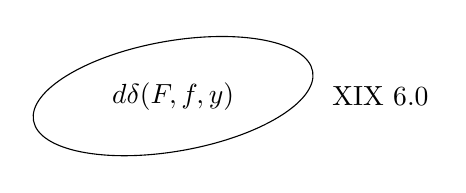
\begin{tikzpicture}
\node at (0,0) {$\deleted{\unsure{d}}\handwritten{\delta}(F,f,y)$};
\draw[rotate=10] (0,0) ellipse (1.8cm and .7cm);
\node[anchor=west] at (1.9,0) {XIX 6.0};
\end{tikzpicture}}

formellement séparable (k-algèbre - )\quad formally separable \inserted{\handwritten{k-}}algebra\quad XIX 6.7.\inserted{\handwritten{0}}

\figure{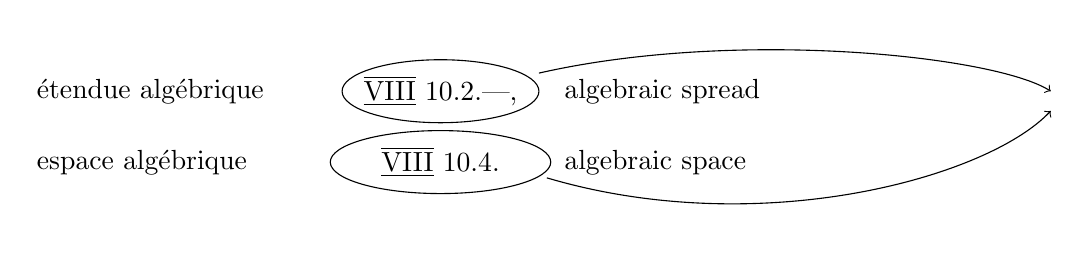
\begin{tikzpicture}
\node[anchor=west] at (0,0) {\handwritten{étendue algébrique}};
\node at (5.25,0) {\handwritten{$\overline{\underline{\mathrm{VIII}}}$ 10.2\unsure{.|,}}};
\node[anchor=west] at (6.7,0) {\handwritten{algebraic spread}};
\node[anchor=west] at (0,-.9) {\handwritten{espace algébrique}};
\node at (5.25,-.9) {\handwritten{$\overline{\underline{\mathrm{VIII}}}$ 10.4.}};
\node[anchor=west] at (6.7,-.9) {\handwritten{algebraic space}};
\draw (5.25,0) ellipse (1.25cm and .4cm);
\draw (5.25,-.9) ellipse (1.4cm and .4cm);
\draw[->] (6.5,.23) .. controls (9,.8) and (12.3,.45) .. (13,0);
\draw[->] (6.6,-1.1) .. controls (9.3,-1.9) and (12.2,-1.1) .. (13,-.25);
\end{tikzpicture}}
% archive sheet number: 44
